
\chapter{Scenarios}
This section briefly discuss some of the scenarios : A content distribution
example, an Augmented Internet and a personal mobile scenario. They were chosen to
represent different perspectives of the possibilities of the NetInf approach. Each scenario is
discussed with the problem it is addressing, some of the requirements it puts on NetInf as well
as the advantage such a scenario will obtain when combined with NetInf.

\section{Content distribution}

Contemporary content distribution has effectively become an assortment of individual and
specialized solutions. Depending on the field of application, these solutions range from
carefully engineered and managed Content Distribution Networks owned by individual corpo-
rations to more ad-hoc and unmanaged peer-to-peer networks such as BitTorrent based
file exchange overlays . In addition, a number of technologies, such as content personal-
ization and adaptation have emerged. Although these technologies seem quite different in the
way they are approaching the problem, effectively they are in fact all dealing with getting
content from information producers to information consumers. It is, therefore, natural to
investigate how to employ Networks of Information in the field of content distribution.
% \begin{figure}[h]
% \begin{center}
% \includegraphics[height=6cm]{9.jpg}
% \caption{Algorithm form for system COSDES}
% \end{center}
% \end{figure}

Here envisage a solution where NetInf provides a uniform mechanism for accessing content,
seamlessly incorporating different content types and distribution methods. These include
novel schemes that either blend existing approaches or define new ones. A key enabler to this
approach is the notion of information objects, a NetInf architecture cornerstone. In this archi-
tecture, the particular representation of information (e.g. a MP3 file) and how it is retrieved
(e.g. HTTP or BitTorrent) are orthogonal to the information object itself.

Using the notion of Information Objects, there is a method that can accommodate different
kinds of distribution schemes and network scenarios. This means that all that is needed is the
identifier of the information object to be retrieved. Given this identifier, the NetInf infrastructure
will then decide what the optimal source or sources are, and deliver the content to the user.
The source in this context is not defined until the retrieval begins. Possible distribution
schemes include simple point-to-point transfers and live streaming as well as more sophisticated P2P methods. The choice may well be determined on whether the object is to be
shared, and by how many potential recipients. The key differentiator to today’s solutions is that
that the whole range of possible distribution mechanisms can be exploited for a given transfer.
Especially in the light of the trend towards high definition video that leads to constantly in-
creasing data volumes, this enables the networks to choose source and distribution mode in
an optimized manner.

But also the classical web browsing can benefit from NetInf technology. Today, many of the
distributed data storage technologies (particularly P2P systems) are not applicable to web
browsing. The setup times associated to a file transfer (e.g. finding and connecting to the
peers) can account for a substantial fraction of the download time, often tens of seconds. For
large downloads, this set-up delay is acceptable, as it only represents a small fraction of the
overall time spent performing the download, however web usage typically requires many
smaller transmissions. Such set-up latencies would mean that the average web page would
take several minutes to load, clearly out of most users’ expectations. As a result of these
latencies, web-browsing maintains a strictly client-server model, with the consequences that
resources are frequently concentrated in one topological region, meaning that availability of
these resources are threatened by any agent capable of disabling or destroying a single
server (peer-to-peer systems are typically able to offer some degree of resilience in this
regard). This envision a Serverless Web which attempts to create a peer-to-peer style system
with latency characteristics which would be considered acceptable for web browsing. The
goal, therefore, is to attempt to develop in NetInf a decentralised method of distributing data,
while minimising the associated coordination latencies.

As further aspects of the work in NetInf, planning is there to explore the benefits of including
network services in the distribution chain, such as different types of content adaptation.
Transcoding, for example, has already been used in the existing Internet where properties
such as the resolution or the bit rate of an information object are changed in real time. Content
personalization, and the required content adaptation, is also increasing in importance. The
actual media processing may also occur external to NetInf, with NetInf selecting the appropri-
ate transport mechanism when available. The cryptographic properties of information objects
can be exploited in order to control access to the information. This embraces the well-known
Digital Rights Management (DRM) scheme already known today to e.g. only grant access to a
media file when a fee has been paid. In addition, the protection of user-generated content is
an important issue to be solved.

\section{Augmented internet}
As mobile Internet-enabled devices become more ubiquitous, users will want to use them to
access greater amounts of information and services in the real world. This includes objects
close to the users such as everyday objects, people they meet, or places they visit. When
accessing information on the move, it is essential that the accessing information does not
detract the user's attention from the real-world activities. Unfortunately, mobile Internet access
as experiencing it today requires a lot of attention by the user and is therefore not suitable
for many scenarios. To support such scenarios, a smooth integration with the real world that
enables service access without interrupting the user's real-world work flow is needed by
Internet applications. However, such applications are difficult to build on a large scale due to
the current Internet architecture. Basically it does not provide a notion for real-world integra-
tion.

The concept of network support for real-world-integrated applications the Augmented
Internet paradigm, for example, a tourist near the Eiffel Tower cares about opening hours,
ticket cost, the history of the monument, and so on. Whether this information is located on a
server in Paris or elsewhere is irrelevant to the user. URIs such as www.tour-eiffel.fr provide
an abstraction layer to the location of information, but nevertheless tie it to specific network
nodes.  Real-world integrated applications are inherently information-centric and
that NetInf is well suited to provide an architecturally sound infrastructure to enable and
support real-world-integrated applications. Such applications pose two main requirements on
an underlying infrastructure. First, the Augmented Internet needs a notion of virtual represen-
tations for physical entities that can cumulate and provide access to physical-entity-related
services. Second, the Augmented Internet has to build and maintain a binding between the
physical entity and its virtual representation on the future Internet. The NetInf architecture
addresses these requirements by providing an API that is common for objects that represent
real-world entities as well as objects that represent services, content, and other digital entities.
Based on the common API and the information model, bindings and interactions can be
defined between the objects representing real-world and digital entities to enable Augmented
Internet applications.
The Augmented Internet paradigm combines multiple families of use cases that are described
next. One family combines use cases that enable the interaction with physical entities via
entity-related Internet services directly from the real world. This facilitates a completely new
real-world interface to access physical-entity-related services without the need for a conven-
tional Internet search. A tourist could, for example, obtain information about buildings and
places by simply pointing with his cellular phone at a building instead of performing a cumber-
some full-text search. Any output interface like an audio headset or the cell phone display
could be used to unobtrusively present the resulting information as illustrated in Figure 2. In
this use case, identifying the monument can technically be realized by using physical attrib-
utes of the building such as its estimated GPS position, via the users position and an elec-
tronic compass. These attributes will be used by the Augmented Internet infrastructure to build
and maintain a connection between entity-related information and the physical entity itself.

 \begin{figure}[h]
 \begin{center}
 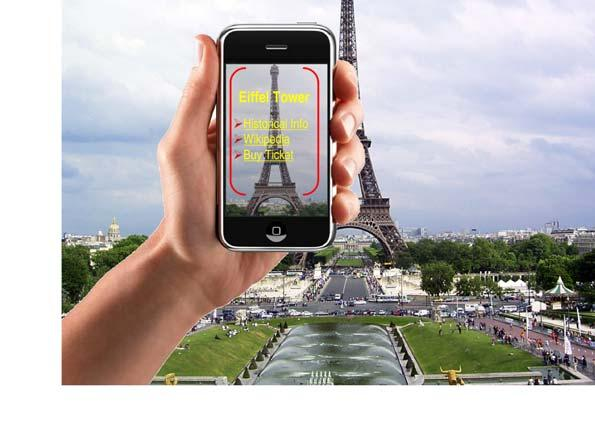
\includegraphics[height=6cm]{4.jpg}
 \caption{Tourist application: Accessing information about buildings}
 \end{center}
 \end{figure}

Similarly an Augmented Internet service could identify objects based on, for example, Radio
Frequency Identification (RFID) tags and could execute Internet services related with the
referenced object. For example, a user could ``click on'' a library book, thereby executing the
online service to renew the book. Furthermore, a selection menu could be displayed to the
user, providing additional options like accessing the bibliographic information of the book. All
book-related information are cumulated in the book's virtual representation, provided and
maintained by the information-centric network infrastructure. A simple Augmented Internet
service could also enable a user to store personal notes in this virtual representation, hence
directly binding them to the book instead of storing the notes in some separated text document that can be difficult to retrieve.

Furthermore, an Augmented Internet could enable people to use web methods such as
bookmarking in the real world: a user could bookmark interesting products by ”clicking” on the
physical object with a cell phone. Likewise, a user could add a virtual post-it to a specific
object by the same method.

\section{Personal Mobile Scenario}
A person on the move is a common scenario for many projects investigating new ideas for
improving communication in a mobile and wireless environment. Past projects have looked at
composing networks, seamless integration of multiple radio technologies and various other
multi-access mechanisms. Most solutions however cannot handle frequent disconnec-
tions because they rely on that there always is enough connectivity to keep an end-to-end
TCP connection alive.

In the NetInf personal mobile scenario, disruptions and disconnections for shorter or longer
times are important characteristics making it different from previous projects. The argument is
that it is impossible to provide good wireless service everywhere and therefore also in
the future often will experience disruptions when communicating on the move. The purpose
with the scenario is to show that the NetInf approach can provide better service under these
conditions compared to current technology by circumventing the need for end-to-end connec-
tions and making use of intermediate storage, much in the same way as Delay Tolerant
Networking (DTN) does. The extreme case is when there never is connectivity simultaneously
along the end-to-end path.

In the personal mobile scenario, a person is using a laptop to read and send email while
travelling on a train as illustrated in Figure 3.2. The train passes stations now and then where
local hot-spots with high-speed wireless communication are available. The hot-spots also
have storage that the NetInf functionality can use temporarily. In addition to the hot-spots,
cellular service (3G) is available with varying quality during the journey. The varying quality
can have a severe impact on the application performance experienced by the user.

On the down-link to the train NetInf can make full use of the hot-spot capacity by prefetching
desired information before the train arrives, and on the up-link by quickly offloading informa-
tion to the storage and later relay to the final destination. The goal for NetInf in this scenario is
to make the best use of both the cellular and the hot-spot capacity.


\begin{figure}[h]
 \begin{center}
 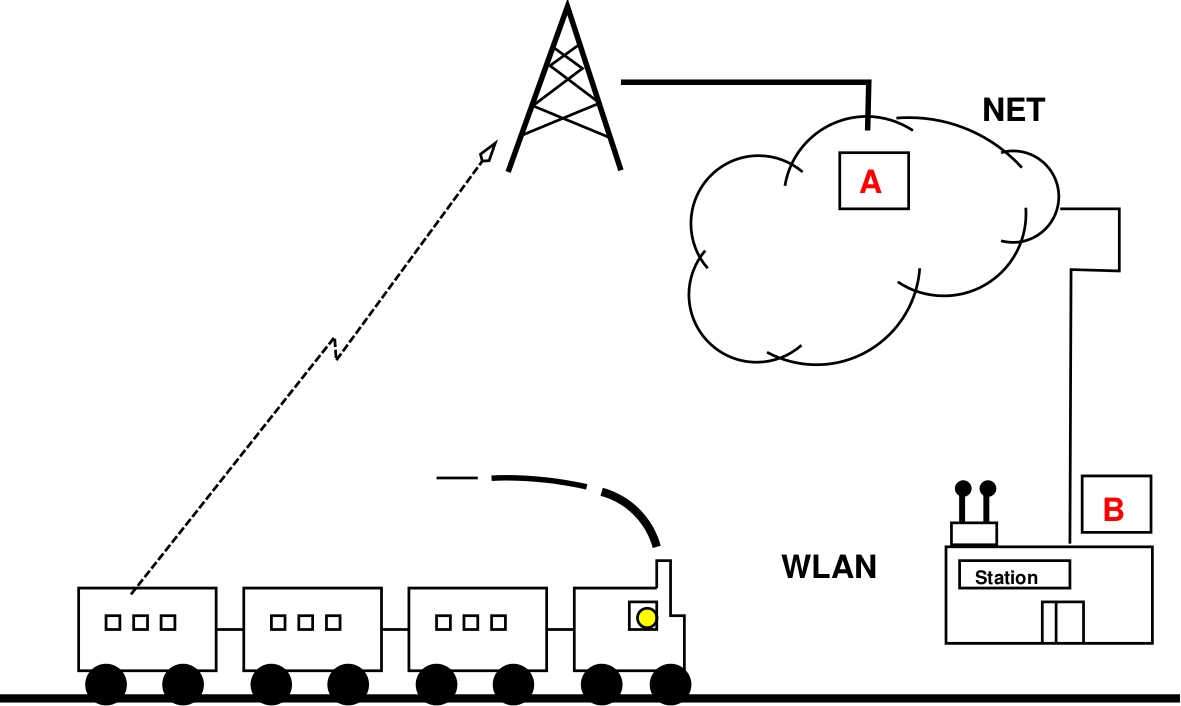
\includegraphics[height=6cm]{5.jpg}
 \caption{Personal Mobile Scenario}
 \end{center}
 \end{figure}

The scenario proceeds as follows:
\begin{itemize}
 \item The user initiates email retrieval from the mailbox at A over the cellular radio link.
 \item The system concludes that retrieval will take a long time due to insufficient capacity, possibly caused by disruptions.
 \item The system determines that the next available hot-spot is at station B.
 \item A is instructed to send the mailbox to the storage at B.
 \item The train arrives at B and the user can quickly receive the remaining part of the mailbox.

\end{itemize}


An alternative is that the user communicates directly with B through the cellular link and sends
a pre-fetch message to B. B would then pull the data from A on the user’s behalf. To achieve
this, the network must have the ability to locate the closest copy of an object and be able to
move the data closer to where the user will be soon. This replication may either be triggered
by some (low-bandwidth) control message or automatically by the network. Also, either the
network or the client needs a way to predict which stations would be suitable to replicate data
to. Such network primitives would provide benefits to the current synchronous Internet model,
by providing an asynchronous model of communication to mobility aware applications. This
would also allow decoupling of the wanted information from the originating nodes. It would
finally provide bandwidth adaptation and improve usage enabling the use of transient access.


